\section{Polymere Stoffe: Kunststoffe}
\subsection{Allgemeines zu polymeren Stoffen}
Polymere Stoffe bestehen aus Molekülen, die aus sehr vielen gleichen oder unterschiedlichen kleinen Molekülen, sog. Monomeren, aufgebaut sind. Die molare Masse liegt oft über 10'000 g/mol. Makromoleküle lassen sich in kleine, sich wiederholende Abschnitte, \emph{Monomere}, unterteilen. \\

Polymere Stoffe lassen sich unterteilen in:
\begin{itemize}
	\item Naturstoffe, z.B. Baumwolle, Stärke, Kautschuk
	\item umgewandelte Naturstoffe, z.B. Gummi, Kunsthorn
	\item synthetische Stoffe (Kunststoffe), z.B. Polyethen PE, Polyvinylchlorid PVC
	\begin{itemize}
		\item Thermoplaste (lineare oder verzweigte Makromoleküle)
		\item Duroplaste (engmaschig vernetzte Makromoleküle)
		\item Elastomere (weitmaschig vernetzte Makromoleküle)
	\end{itemize}
\end{itemize}

\begin{figure}[htbp]
	\centering
	\begin{subfigure}{0.25\linewidth}
		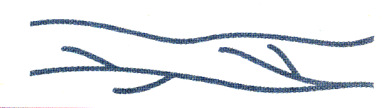
\includegraphics[width=0.9\linewidth]{images/7_Thermoplast}
		\caption{Thermoplast}
	\end{subfigure}
	\quad
	\begin{subfigure}{0.25\linewidth}
		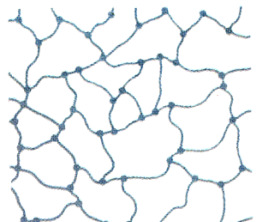
\includegraphics[width=0.9\linewidth]{images/7_Duroplast}
		\caption{Duroplast}
	\end{subfigure}
	\quad
	\begin{subfigure}{0.25\linewidth}
		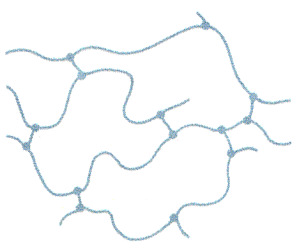
\includegraphics[width=0.9\linewidth]{images/7_Elastomer}
		\caption{Elastomer}
	\end{subfigure}
\end{figure}

\subsection{Typische Eigenschaften von Kunststoffen}
\begin{itemize}
	\item Geringe Dichte (0.8 bis 2 g/cm$^3$), weil Atome vor allem aus C \& H-Atomen bestehen (geringe Masse).
	\item Geringe thermische und elektrische Leitfähigkeit, weil keine geladenen, frei beweglichen Teilchen vorhanden sind.
	\item Grosse Korrosionsbeständigkeit, weil keine reaktionsfreudigen Gruppen.
	\item Niedrige Verarbeitungstemperaturen
	\item Flexible Elastizitätsmodule und Zugfestigkeit
	\item Geringe Temperaturbeständigkeit
	\item Kein definierter Schmelzpunkt sondern Erweichung, weil sie nicht bei einer bestimmten Temperatur sondern innerhalb eines Temperaturbereichs schmelzen $\rightarrow$ Kristallinität der Thermoplaste
	\item Kein Siedepunkt, sondern Zersetzung, weil VdW-Kräfte oder Vernetzung
\end{itemize}

\subsection{Thermoplaste}
Bsp. Polyethen (PE), Polypropen (PP), Polyvinylchlorid (PVC), Polyethylenterephthalat (PET), ... 

\subsubsection{Der Atomare Aufbau von Thermoplasten}
Thermoplaste bestehen aus kettenartigen Makromolekülen, welche linear (unverzweigt) oder verzweigt sein können.\\Molare Masse: $10^4$ bis $10^6$g/mol. Länge Makromolekül: $10^{-6}$ bis $10^{-3}$mm. Kettenlänge kann innerhalb des Polymers variieren. Die mittlere Anzahl der in den Makromolekülen enthaltenen Monomere heisst Polymerisationsgrad.

\subsubsection{Kristallinität bei Thermoplasten}
Thermoplaste sind teilkristallin, d.h. es können kristalline (relativ geordnet) und amorphe (wirr ineinander) Bereiche vorkommen.

\subsubsection{Taktizität bei Thermoplasten}
Taktizität bezeichnet die räumliche Anordnung der Seitenketten in verzweigten Makromolekülen (kann bei Herstellung beeinflusst werden).

\begin{figure}[htbp]
	\centering
	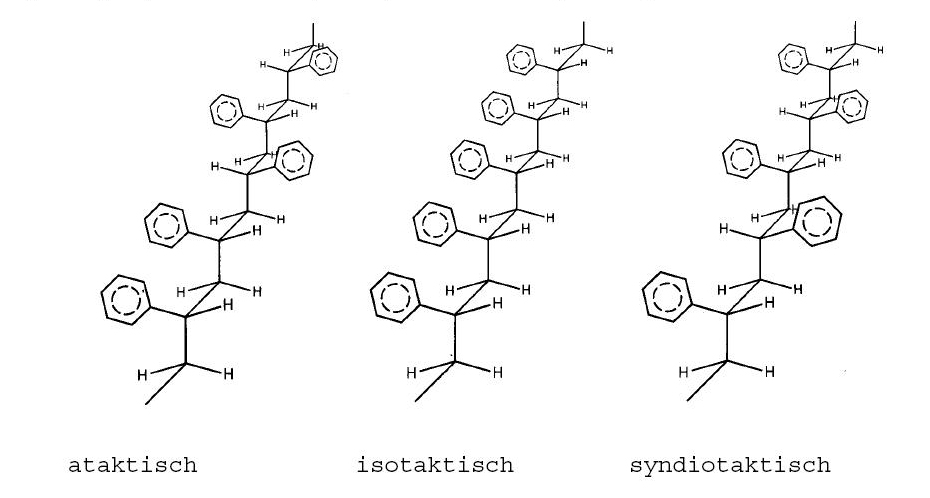
\includegraphics[width=0.7\linewidth]{images/7_Taktizitaet.png}
\end{figure}

\begin{itemize}
	\item ataktisch: Seitengruppen liegen regellos auf der einen oder der anderen Seite $\rightarrow$ amorphe Kunststoffe
	\item isotaktisch: alle Seitengruppen sind nach einer Seite ausgerichtet $\rightarrow$ hoher Kristallinitätsgrad möglich
	\item syndiotaktisch: Seitengruppen liegen in regelmässiger Abfolge auf der einen und der anderen Seite der Hauptkette
\end{itemize}

\subsubsection{Typische Eigenschaften der Thermoplaste}
\begin{itemize}
	\item schlecht löslich (nur in bestimmten organischen Lösungsmitteln) oder unlöslich (VdW-Kräfte)
	\item Durchlaufen beim Erwärmen versch. Aggregatzustände: fest $\rightarrow$ thermoelastisch (Formänderung umkehrbar) $\rightarrow$ thermoplastisch (Formänderung nicht umkehrbar) $\rightarrow$ flüssig $\rightarrow$ Zersetzung
	\item Grad der Kristallinität beeinflusst Eigenschaften stark. Je kristalliner, desto härter, dichter und weniger löslich. Zudem weisen sie geringere Wärmebeständigkeit auf.
\end{itemize}

\subsection{Duroplaste}
Bsp. Phenoplaste PF (Isoliermaterial, Steckdosen), Aminoplaste (Spannplattenleim), Ungesättigte Polyesterharze UP, Epoxidharze EP
\subsubsection{Der Atomare Aufbau von Duroplasten}
Duroplaste bestehen aus Makromolekülen, die durch Atombindungen räumlich engmaschig vernetzt sind $\Rightarrow$ hart, spröde, zerbrechlich, hitzebeständig (Netzstruktur bleibt beim Erwärmen erhalten) bis zur Zersetzung.

\subsection{Elastomere}
Bsp. Vernetze Polyurethane (PUR), Naturkautschuk (NR), Chloropren-Kautschuk (CR), Silikon-Kautschuk
\subsubsection{Der Atomare Aufbau von Elastomeren}
Elastomere bestehen aus räumlich weitmaschig verknüpften Makromolekülen $\Rightarrow$ elastisch, Zersetzung bei starkem Erwärmen

\subsection{Herstellung von Polymeren}
\subsubsection{Polymerisation} 
Verknüpfung der Monomere unter Spaltung einer Doppelbindung und Bildung einer neuen Einfachbindung $\Rightarrow$ kettenartige Makromoleküle $\Rightarrow$ Thermoplaste \\
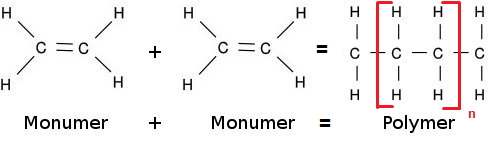
\includegraphics[width=9cm]{images/Polymerisation.png}

\subsubsection{Vulkanisation}
Vernetzung von Makromolekülen mit Doppelbindungen. Ablauf: Zugabe von Schwefel $S_8$, Spaltung der $S_8$-Moleküle, Vernetzung der Makromoleküle, Produkt wird elastisch. 